\section{Actuation System}
The actuation system present on the vessel is constituted by the thrusters and the ESCs.

\subsection{Thrusters}
The thrusters are the main actuators present on the vessel and they provide a forward force depending on the rotational speed of the motors.

The relationship between the command and the force that they exert have been obtained through an experimental test described in \autoref{app:forceTest}. It is as follows
%
\begin{flalign}
    \mathrm{PWM} = \num{6.6044} \ F + \num{70.0168} \ \ .
    \label{eq:backwardSpeedForce}
\end{flalign}
%
If a negative force is required, they can also rotate in the opposite direction, producing a backwards force that is calculated as 
%
\begin{flalign}
    \mathrm{PWM} = \num{8.5706} \ F - \num{91.9358} \ \ .
    \label{eq:forwardSpeedForce}
\end{flalign}
%

The thrusters are actuated with brushless motors INLINE 750 \num{14.8} V from Graupner. They have two poles with a velocity constant of 1035 rpm$\cdot$kV$^{-1}$ and can operate within \num{7.4} and \num{22.2} V, being the nominal voltage \num{14.8} V. \cite{motors}

\begin{figure}[H]
    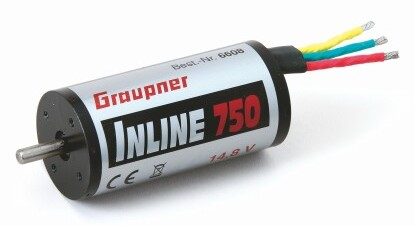
\includegraphics[width=0.4\textwidth]{figures/motor}
    \caption{INLINE 750 \num{14.8} V motor used to produce the thrust in the surface vessel \cite{motors}.}
    \label{fig:motors}
\end{figure}

\subsection{Electronic Speed Controllers}
In order to have the motors turning to the desired rotational speed, electronic speed controllers (ESCs) +70 G\num{3,5} from Graupner are used. The supply voltage ranges from 6 to 25 V and they can handle up to 70 A in continuous current. The reference PWM that comes from the microcontroller translates into a 32 kHz PWM signal to the motors. \cite{ESC}

\begin{figure}[H]
    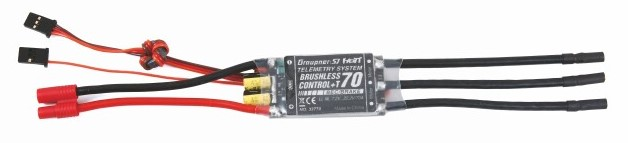
\includegraphics[width=0.8\textwidth]{figures/ESC}
    \caption{Speed controllers +70 G\num{3,5} used to control the  thrusters in the surface vessel \cite{ESC}.}
    \label{fig:ESC}
\end{figure}

%\subsection{Side Thrusters}
%The side thrusters move the vessel sideways but their influence in its motion is limited to low speed maneuvers and they are intended for fine positioning of the vessel. For this reason, they are not utilized in the controller design of the vessel.
